\documentclass[journal,onecolumn]{IEEEtran}
\usepackage[utf8]{inputenc}
\usepackage[T1]{fontenc}
\usepackage[spanish,es-tabla]{babel}
\usepackage{graphicx,amsmath,amssymb,booktabs,tabularx,array,float,cite}
\usepackage[section]{placeins}
\usepackage[hidelinks]{hyperref}
\graphicspath{{figuras/}}
\newcommand{\ucoord}{\,\mathrm{u}}
\newcommand{\figura}[3]{\begin{figure}[H]\centering\includegraphics[width=.97\linewidth,height=.43\textheight,keepaspectratio]{#1}\caption{#2}\label{#3}\end{figure}}
\renewcommand{\arraystretch}{1.14}
\setlength{\emergencystretch}{2em}
\renewcommand{\IEEEkeywordsname}{Palabras clave}
\begin{document}
\title{Segmentación multietapa de una instalación industrial mediante conectividad espacial, atributos locales y verificación geométrica}
\author{Sebastian Chu Lama, Farid Espinoza Pachas, Sofia Valentina Ku Paredes,\\Marcia Sofia Arce Montesinos y Alessandra Lopez-Ameri Castro\\Grupo 10 --- Ingeniería de Computación\\Universidad de Ingeniería y Tecnología (UTEC), Lima, Perú}
\maketitle
\begin{abstract}
En una nube de puntos industrial, separar los objetos no siempre es sencillo porque muchas estructuras están muy cerca o incluso se tocan. En esta actividad estudiamos una nube de 1\,647\,021 puntos con posición, color y normales mediante un procedimiento no supervisado de varias etapas. Se emplean voxelización trazable, planos RANSAC, DBSCAN, conectividad restringida por atributos y refinamientos locales. La verificación de secciones circulares añade siete conducciones cilíndricas candidatas y una comprobación semántica conservadora recupera seis regiones desconocidas. Comparamos distintos parámetros para estudiar cuándo el método separa mejor las estructuras y cuándo termina uniendo objetos diferentes. La salida conserva todos los puntos y su orden, contiene 1\,967 regiones y alcanza 97,08\% de cobertura de instancias. La región mayor ocupa 14,96\% del escaneo, frente a 74,69\% en la referencia espacial seleccionada; 25,03\% de los puntos mantiene clase desconocida. La revisión visual de casos seleccionados permitió identificar errores de clasificación, regiones incompletas y posibles uniones entre objetos distintos. El procesamiento y los resultados se documentan en un notebook reproducible. Persisten limitaciones en conexiones, objetos complejos y categorías ausentes del clasificador geométrico.
\end{abstract}
\begin{IEEEkeywords}Nubes de puntos, segmentación por instancias, agrupamiento no supervisado, geometría local, RANSAC, DBSCAN.\end{IEEEkeywords}

\section{Introducción}
Las instalaciones industriales contienen numerosas estructuras que se encuentran muy cerca unas de otras. En una fábrica podemos encontrar columnas, vigas, tuberías, maquinaria y otras piezas que se cruzan o están conectadas. Aunque para una persona resulte relativamente sencillo distinguirlas al observar la escena, el problema cambia cuando solo contamos con una nube de puntos 3D. Cada punto proporciona información sobre su posición, color y orientación, pero no indica directamente a qué objeto pertenece.

Por ejemplo, una tubería puede pasar junto a una viga o apoyarse sobre una estructura metálica. Si agrupamos sus puntos únicamente por cercanía, ambos elementos podrían terminar dentro de una misma región. También puede ocurrir lo contrario. Un solo objeto puede quedar dividido en varios segmentos debido a espacios sin puntos, cambios de orientación o diferencias en la densidad del escaneo. Por eso, además de la distancia, necesitamos considerar otras características de la geometría.

En este trabajo desarrollamos un procedimiento de segmentación no supervisada para una instalación industrial representada por 1\,647\,021 puntos. Nuestro objetivo fue separar sus principales estructuras y asignar categorías geométricas cuando fuera posible, conservando la nube original y exportando los resultados en formato PLY. Para ello combinamos diferentes métodos. Primero simplificamos los datos, después identificamos superficies grandes y finalmente procesamos las regiones más complejas mediante agrupamiento, análisis de vecinos y refinamientos geométricos.

También comparamos distintas configuraciones para entender cómo influyen sus parámetros en el resultado. No buscamos únicamente obtener más segmentos, ya que un mayor número de regiones también podría indicar que estamos dividiendo innecesariamente los objetos. Por ese motivo, analizamos tanto la cantidad de puntos agrupados como la separación de estructuras y complementamos las métricas con una revisión visual de casos específicos.

La Fig.~\ref{fig:entrada} muestra la nube original. En ella se observa una cubierta elevada sostenida por columnas, junto con una zona de tuberías y estructuras metálicas más pequeñas. La cantidad de conexiones entre estos elementos explica por qué resulta difícil resolver toda la escena con un solo algoritmo.
\figura{entrada.png}{Nube original de la instalación industrial, representada con los colores RGB del escaneo. Se distinguen la cubierta superior, las columnas de soporte y la zona frontal con tuberías y estructuras metálicas, donde existen numerosos puntos de contacto.}{fig:entrada}
La vista permite identificar estructuras de tamaños muy distintos y zonas donde varias piezas se superponen visualmente. En las secciones siguientes describimos los métodos utilizados, los experimentos realizados para elegir sus parámetros y los resultados obtenidos en la segmentación y clasificación final.

\section{Marco teórico}
\subsection{Atributos y significado de las salidas}
Una nube de puntos representa una escena mediante posiciones $\mathbf{x}_i\in\mathbb{R}^3$ tomadas sobre sus superficies. El color RGB aporta información visual, mientras que las normales indican hacia dónde está orientada cada superficie en un entorno pequeño. Combinar varias características para describir los datos es una práctica habitual en reconocimiento de patrones \cite{bishop,muller}. El color puede variar por iluminación y la normal puede cambiar de signo sin que cambie el plano tangente. Por eso ambos atributos son pistas geométricas o visuales, no identificadores de objeto. Open3D proporciona operaciones de procesamiento tridimensional utilizadas en el proyecto, entre ellas el ajuste de planos \cite{open3d}.

Trabajamos con dos resultados relacionados. La segmentación por instancias reúne puntos dentro de regiones y asigna un identificador a cada una. La clasificación semántica intenta indicar qué tipo de estructura representa una región. Así, dos fragmentos de una columna pueden pertenecer a instancias diferentes y compartir la categoría de soporte vertical. También puede haber regiones bien delimitadas cuya clase siga siendo desconocida porque su forma no aporta suficiente información. Esta diferencia será importante al analizar los errores del resultado final.

\subsection{Voxelización}
La voxelización divide el espacio en celdas cúbicas y representa cada celda ocupada mediante un agregado de sus muestras. Para un lado $v$ y un origen $\mathbf{o}$ se calcula
\begin{equation}\mathbf{k}_i=\left\lfloor(\mathbf{x}_i-\mathbf{o})/v\right\rfloor,\qquad \ell_i=\widehat{\ell}_{m(i)}.\label{eq:voxel}\end{equation}
En la Ec.~\eqref{eq:voxel}, $\mathbf{k}_i$ es la celda del punto, $m(i)$ es el índice de su representante, $\widehat{\ell}$ es la etiqueta reducida y $\ell_i$ es la etiqueta recuperada en el orden original. El mapeo evita una transferencia aproximada por vecino más cercano. La simplificación reduce consultas espaciales, pero puede promediar detalles que comparten una celda. Conservar las filas originales no recupera una separación que ya se perdió dentro de un voxel.

\subsection{Principal Component Analysis(PCA)}
El PCA o análisis de componentes principales permite estudiar cómo se distribuyen los puntos en distintas direcciones. En una nube 3D nos ayuda a reconocer si una región tiene forma alargada, se parece a una superficie plana o presenta volumen en varias direcciones. Para ello analiza la dispersión de los puntos alrededor de su centro. Con $k$ vecinos $\mathcal{N}_i$ y centro $\boldsymbol{\mu}_i$ se calcula
\begin{equation}C_i=\frac{1}{k}\sum_{j\in\mathcal{N}_i}(\mathbf{x}_j-\boldsymbol{\mu}_i)(\mathbf{x}_j-\boldsymbol{\mu}_i)^T.\label{eq:pca}\end{equation}
Los autovectores de la matriz de covarianza de la Ec.~\eqref{eq:pca} señalan las direcciones en las que los puntos varían más o menos. Ordenando los autovalores como $0\leq\lambda_0\leq\lambda_1\leq\lambda_2$, la implementación obtiene
\begin{equation}L=\frac{\lambda_2-\lambda_1}{\lambda_2},\quad P=\frac{\lambda_1-\lambda_0}{\lambda_2},\quad c=\frac{\lambda_0}{\lambda_0+\lambda_1+\lambda_2}.\label{eq:shape}\end{equation}
En la Ec.~\eqref{eq:shape}, $L$ es linealidad, $P$ planaridad y $c$ una medida de variación superficial utilizada como curvatura. En los cálculos se evita dividir entre valores cercanos a cero. Cuando casi todos los puntos siguen una dirección, como en un tramo de viga, aumenta $L$. Si se distribuyen sobre dos direcciones, como en un panel, aumenta $P$. En cambio, si también se dispersan en la tercera dirección, crece $c$, que aquí utilizamos como una aproximación de la variación de la superficie y no como una medida exacta de curvatura. Los descriptores basados en autovalores se emplean habitualmente para caracterizar vecindarios 3D \cite{demantke}. PCA también se utiliza para reducir dimensiones y estudiar la variación de datos en aprendizaje automático \cite{bishop,muller}. En nuestra implementación se usa un tamaño fijo de 20 muestras.

\subsection{RANSAC y DBSCAN}

RANSAC (\textit{Random Sample Consensus}) intenta encontrar un modelo geométrico, como un plano, usando pequeñas muestras de puntos. Después comprueba cuántos de los demás puntos se ajustan al modelo \cite{ransac}. Para un plano de normal unitaria $\mathbf{a}$ y desplazamiento $b$, un punto es compatible si $|\mathbf{a}^T\mathbf{x}_i+b|<\tau$, donde $\tau$ es la tolerancia espacial. Un umbral amplio incorpora más muestras, pero también puede absorber objetos próximos; uno estrecho puede dejar bordes o superficies imperfectas sin asignar. Más iteraciones aumentan las oportunidades de proponer un modelo útil, sin demostrar que los puntos aceptados pertenezcan al mismo objeto.

DBSCAN (\textit{Density-Based Spatial Clustering of Applications with Noise}) agrupa puntos según su densidad local. Para hacerlo utiliza un radio $\varepsilon$ y una cantidad mínima de puntos, \texttt{MinPts}. Un punto núcleo tiene suficientes muestras dentro del radio, contando la propia muestra; uno de borde pertenece a la vecindad de un núcleo sin cumplir ese mínimo; el ruido queda fuera de los grupos alcanzados. El algoritmo conecta zonas densas sin fijar su número de antemano \cite{dbscan}. Esa conectividad permite formas irregulares, pero también atraviesa una cadena de contactos entre objetos distintos. Aumentar $\varepsilon$ o reducir \texttt{MinPts} facilita esa unión; restringirlos puede fragmentar zonas poco densas.

\subsection{Grafos, orientaciones y modelos cilíndricos}
Un grafo nos permite representar cada punto como un nodo y conectar únicamente los pares de vecinos que cumplen ciertas condiciones. En nuestro método, las aristas cumplen simultáneamente límites de distancia, orientación de normales, diferencia RGB, curvatura y separación respecto al plano tangente. No se suman coordenadas, colores y ángulos en una distancia conjunta. Cada magnitud se compara con un umbral en su propia escala y las componentes conexas definen regiones.

MiniBatchKMeans actualiza centros con lotes pequeños y aproxima el objetivo de agrupar observaciones por cercanía a dichos centros \cite{sculley}. En nuestro procedimiento lo usamos solo para dividir temporalmente las regiones grandes según la orientación de sus puntos. Sus diez grupos no representan diez clases ni diez objetos. La representación simétrica $\mathbf{n}\mathbf{n}^T$ evita distinguir $\mathbf{n}$ y $-\mathbf{n}$; después de esa partición se vuelve a comprobar conectividad espacial.

Un cilindro requiere una sección circular y continuidad longitudinal. Para un centro $\mathbf{p}$, eje unitario $\mathbf{a}$ y radio $r$, el residuo radial es
\begin{equation}e_i=\left|\left\|(\mathbf{x}_i-\mathbf{p})-\big((\mathbf{x}_i-\mathbf{p})^T\mathbf{a}\big)\mathbf{a}\right\|-r\right|.\label{eq:cylinder}\end{equation}
La Ec.~\eqref{eq:cylinder} calcula la distancia de cada punto al eje del cilindro y comprueba cuánto se diferencia del radio esperado. Un residuo pequeño sobre una franja no basta para reconocer una tubería. Exigimos soporte de sección y consistencia en varias posiciones. Incluso un modelo aceptado mantiene una etiqueta candidata, pues la forma no confirma por sí sola la función industrial.

\section{Datos y análisis exploratorio}
\subsection{Características verificadas}
El archivo \texttt{FARO\_Scan\_Full\_Sub1\_down3\_with\_normals.ply} contiene 1\,647\,021 puntos. XYZ y normales son \texttt{float32}; RGB se almacena como tres canales \texttt{uint8}. No se registraron coordenadas duplicadas ni atributos no finitos y aparecen dos normales nulas. No se descartan puntos del resultado por esos dos casos; las normalizaciones protegen la división por cero.

La caja del escaneo mide aproximadamente $31,386\times34,868\times16,770\ucoord$. El archivo no certifica metros, por lo que utilizamos unidades de coordenadas, u. La dirección vertical estimada difiere solo $0,339^\circ$ del eje Z. Por esa razón, utilizamos Z para analizar alturas y distinguir zonas superiores e inferiores. Esto no significa que el escáner haya proporcionado una medición directa de la gravedad.
\figura{eda_distribuciones.png}{Distribuciones completas de posiciones y canales RGB. Los ejes espaciales se expresan en u; los canales de color, entre 0 y 255.}{fig:distribuciones}
La Fig.~\ref{fig:distribuciones} muestra seis histogramas. En la fila superior aparecen las coordenadas X, Y y Z. Los picos indican posiciones donde se concentra una mayor cantidad de puntos. En Z, por ejemplo, destacan alturas asociadas con superficies grandes, como el piso y las zonas elevadas. En X e Y los puntos se distribuyen de forma desigual porque el escáner registra las superficies de los objetos y no todo el espacio vacío entre ellos. La fila inferior presenta los canales rojo, verde y azul. Sus distribuciones tampoco son uniformes, pero un mismo color puede aparecer en objetos diferentes. Esto nos llevó a utilizar el RGB como información complementaria, sin depender exclusivamente de él para separar estructuras.

\subsection{Orientación y escala de vecindad}
Se conservó una muestra reproducible de 60\,000 consultas sobre la nube original, con semilla 42. La mediana de distancia al primer vecino fue $0,03355\ucoord$ y al octavo $0,06502\ucoord$. El percentil 99 del vecino 16 alcanzó $0,16832\ucoord$, mostrando una cola de regiones menos densas que el comportamiento central.
\figura{eda_normales_vecinos.png}{Distribución de las componentes de las normales (izquierda) y distancias a diferentes vecinos ordenadas por percentiles (derecha). Las curvas permiten comparar la separación habitual entre puntos y detectar zonas menos densas.}{fig:normales}
En el primer gráfico de la Fig.~\ref{fig:normales}, muchas componentes de las normales se encuentran cerca de cero o de uno. Esto es coherente con la presencia de superficies orientadas principalmente a lo largo de los ejes de la escena. Las curvas de distancia se mantienen relativamente bajas durante gran parte de los percentiles y crecen al acercarse al extremo. Por tanto, un radio que conecte zonas dispersas también puede superar ampliamente la separación habitual de muestras en superficies densas. El producto escalar de la Fig.~\ref{fig:producto} se acumula cerca de uno, pero existe una fracción de signos opuestos de 0,263\% en las consultas. Comparar su valor absoluto evita tratar esos signos como una discontinuidad de orientación. Estas distancias nos dieron una referencia para probar los radios de vecindad, aunque por sí solas no indican cuál es el mejor radio para separar objetos.
\figura{producto_escalar.png}{Relación entre las orientaciones de normales vecinas. Los valores cercanos a uno representan direcciones similares; el eje vertical logarítmico permite distinguir los casos menos frecuentes.}{fig:producto}
En la Fig.~\ref{fig:producto}, el pico cercano a uno indica que la mayoría de los vecinos tienen normales orientadas casi en la misma dirección. Los valores próximos a cero corresponden a superficies aproximadamente perpendiculares, mientras que los negativos representan normales que apuntan en sentidos opuestos. El eje vertical utiliza una escala logarítmica porque hay muchísimos más pares cercanos a uno que pares con otras orientaciones. Con una escala normal, las barras pequeñas casi no se verían. Gracias a esta representación podemos observar también esos casos menos frecuentes, que pueden aparecer en cambios de superficie o uniones entre piezas.

\figura{eda_densidad.png}{Densidad de puntos proyectada en XY antes y después de la voxelización (izquierda y centro), y cantidad de puntos originales representados por cada voxel (derecha).}{fig:densidad}
La Fig.~\ref{fig:densidad} compara la distribución de puntos antes y después de la voxelización. Los dos primeros paneles muestran cuántos puntos aparecen en cada zona cuando proyectamos la nube sobre XY. Las zonas más claras tienen mayor concentración, aunque esto también puede ocurrir cuando varias superficies se encuentran una sobre otra a diferentes alturas. El tercer panel indica cuántos puntos originales quedaron representados por cada voxel. La mayoría de celdas contiene pocos puntos, mientras que algunas concentran más muestras. Por ello, cuando calculamos porcentajes sobre la nube reducida, tomamos en cuenta cuántos puntos originales representa cada celda.

\section{Desarrollo metodológico y experimentación}
\subsection{Organización del procedimiento}
La Fig.~\ref{fig:diagrama} resume cómo organizamos el procesamiento. La voxelización conserva un mapa de correspondencia y proporciona representantes para calcular atributos locales. RANSAC divide estos datos en superficies extensas y residuo. Sobre el mismo residuo evaluamos una agrupación espacial con DBSCAN y construimos el grafo restringido que alimenta el refinamiento final. Así, DBSCAN sirve como comparación intermedia; sus grupos no son la entrada del grafo.
\begin{figure}[H]
\centering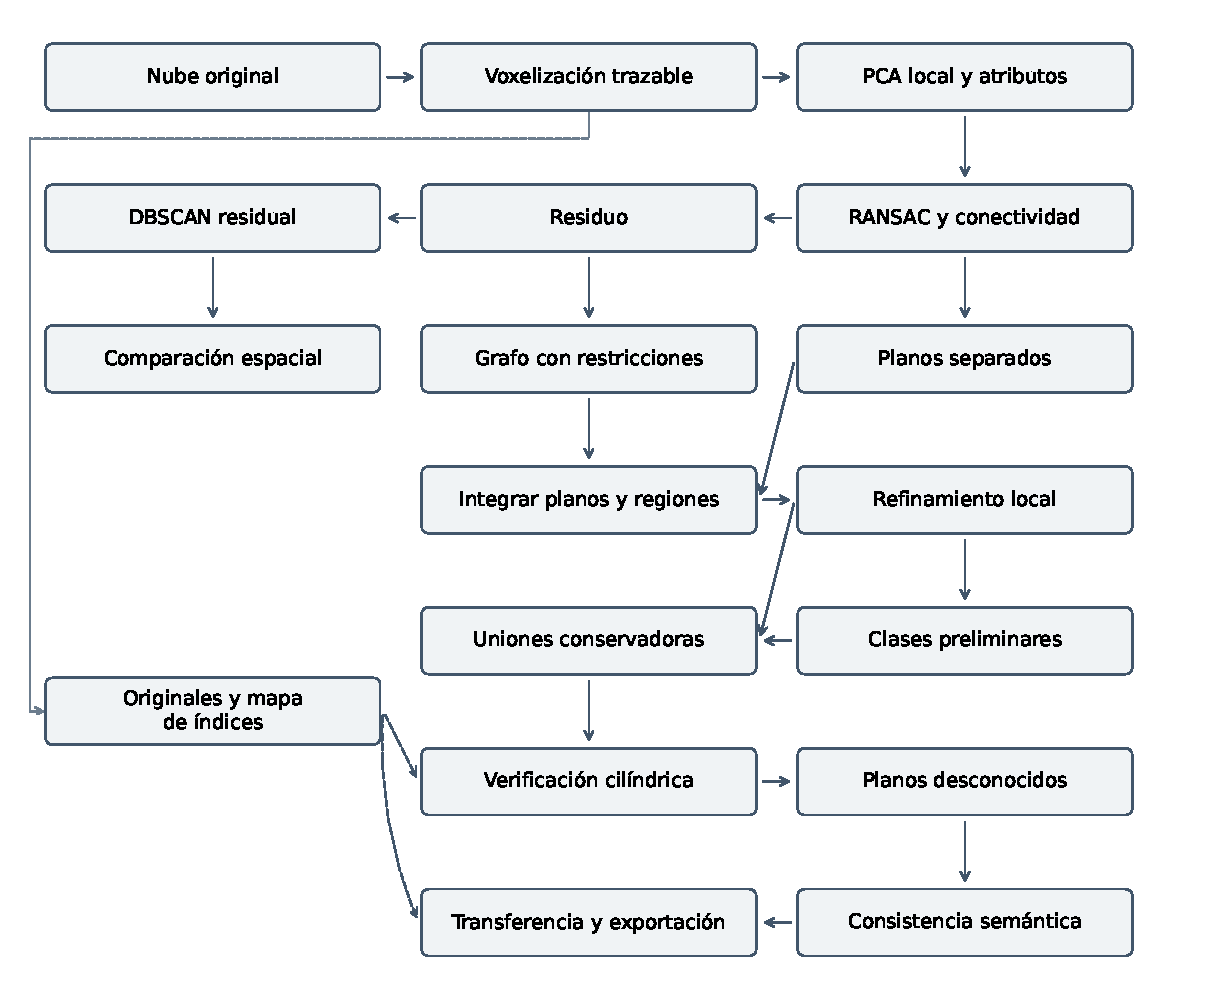
\includegraphics[width=.87\linewidth,height=.55\textheight,keepaspectratio]{diagrama_pipeline.pdf}
\caption{Organización del pipeline. Las ramas de DBSCAN y del grafo comparten el residuo de RANSAC. Las líneas discontinuas indican el uso de los datos originales y del mapa de correspondencia.}\label{fig:diagrama}
\end{figure}
La integración de planos y regiones precede a la división local, la recuperación de bordes y las uniones conservadoras. Las clases preliminares protegen ciertas estructuras durante las uniones; después se verifican cilindros, se comprueban superficies todavía desconocidas y se aplica consistencia semántica. Los originales intervienen en las pruebas transversales y en la exportación, por lo que la nube reducida no sustituye al escaneo de entrada.

Las Tablas~\ref{tab:voxel}--\ref{tab:fragmentos} comparan las variantes de resolución, agrupamiento y refinamiento. Estudiamos cómo cada cambio modifica la cobertura y la concentración de puntos, junto con las diferencias visibles entre particiones. Los tiempos corresponden a cada etapa medida y no se suman como si fueran una única ejecución completa.

\subsection{Representantes y selección del voxel}
Se promedian posiciones y colores por celda. Para las normales se agrega el tensor de orientaciones, en vez de promediar directamente vectores con signos potencialmente opuestos. La Tabla~\ref{tab:voxel} recoge las tres resoluciones conservadas. Los candidatos de filtrado son diagnósticos y no una eliminación automática de todos esos puntos.
\begin{table}[H]
\centering\caption{Resoluciones y candidatos de filtrado registrados. Los tiempos corresponden a cada ensayo.}\label{tab:voxel}
\small
\begin{tabular}{rrrrr}\toprule
$v$ (u) & Representantes & Tiempo (s) & Estadísticos & Por radio\\\midrule
0,06 & 773\,123 & 9,29 & 8\,652 & 3\,550\\
0,08 & 459\,991 & 7,61 & 5\,716 & 1\,980\\
0,12 & 216\,713 & 11,03 & 3\,382 & 1\,133\\
\bottomrule\end{tabular}
\end{table}

El lado de $0,08\ucoord$ reduce el conjunto de trabajo en 72,07\%. Frente a $0,06\ucoord$, elimina 313\,132 representantes adicionales y disminuye el costo de los grafos de vecindad. Pasar a $0,12\ucoord$ vuelve a reducirlos en más de la mitad, pero aumenta el riesgo de promediar caras cercanas de un tubo o una pieza pequeña. Por eso elegimos la resolución intermedia como compromiso entre simplificación y detalle. Los candidatos de filtrado de la Tabla~\ref{tab:voxel} también disminuyen con la resolución, pero ese descenso depende de la nueva densidad y no demuestra que hayan desaparecido errores de adquisición. No se aplicó un descarte general de esos candidatos. Las distancias entre representantes cambian con la operación, de modo que los radios posteriores se interpretan sobre la nube reducida.
\figura{voxelizacion_detalle.png}{Detalle de una estructura con 2\,502 puntos originales y 615 representantes en el mismo recorte. Se usa un color uniforme para comparar la densidad sin introducir diferencias de RGB.}{fig:voxel}
En la Fig.~\ref{fig:voxel} la reducción hace más dispersa la representación conservando la forma global de las caras. La comparación muestra que disminuye la cantidad de puntos procesados, pero mantiene la forma general de la estructura. Esta etapa aún no asigna clases. El mapa definido en la Ec.~\eqref{eq:voxel} permite devolver las etiquetas a todos los puntos originales al terminar el procesamiento.

\subsection{Superficies extensas con RANSAC}
Para detectar las superficies grandes aplicamos RANSAC de manera repetida. El algoritmo intenta encontrar hasta 18 planos y utiliza como máximo 1\,200 iteraciones por ajuste, con una probabilidad objetivo de 0,999. Se exige al menos 700 representantes compatibles, tolerancia $0,055\ucoord$ y alineación de normales dentro de $22^\circ$. Los soportes de cada plano se separan por DBSCAN con radio $0,22\ucoord$ y se conservan componentes de al menos 100 representantes. Por ello un plano matemático puede producir varias regiones físicamente separadas.
\begin{table}[H]
\centering\caption{Variantes de tolerancia de RANSAC sobre el mismo conjunto reducido.}\label{tab:ransac}
\small
\begin{tabular}{rrrrr}\toprule
$\tau$ (u) & Regiones & Cobertura (\%) & Grupo mayor (\%) & Tiempo (s)\\\midrule
0,035 & 75 & 37,92 & 12,30 & 84,19\\
0,055 & 93 & 38,91 & 14,80 & 97,06\\
0,080 & 88 & 41,71 & 18,54 & 67,48\\
\bottomrule\end{tabular}
\end{table}

La Tabla~\ref{tab:ransac} muestra que ampliar la tolerancia de 0,035 a $0,080\ucoord$ aumenta la cobertura de planos de 37,92 a 41,71\% y el grupo mayor de 12,30 a 18,54\%. La cantidad de regiones no aumenta ni disminuye de manera constante al cambiar el umbral. Una tolerancia mayor puede conectar superficies antes separadas y recoger puntos de piezas próximas; una pequeña deja más residuo. El aumento de cobertura entre los extremos es de 3,79 puntos porcentuales, mientras la mayor región crece 6,24 puntos. Este comportamiento sugiere que la tolerancia no solo recupera pequeñas desviaciones de una superficie, sino que también puede ampliar conexiones. La separación de componentes y la comprobación de normales limitan ese efecto, aunque no lo eliminan. Elegimos $0,055\ucoord$ para mantener un soporte amplio sin alcanzar la concentración de la tolerancia mayor. Los tiempos también varían entre las pruebas. Esto ocurre porque, al cambiar la tolerancia, RANSAC acepta distintos conjuntos de puntos y deja una cantidad diferente de datos por procesar en las siguientes búsquedas.
\figura{planes.png}{Resultado de la extracción de planos con RANSAC y separación de componentes. Los colores distinguen regiones planas detectadas; el gris identifica los puntos que se procesarán en las siguientes etapas.}{fig:planos}
En la Fig.~\ref{fig:planos} se observan primero las superficies más extensas, especialmente las zonas del techo y del suelo, mientras que una gran parte de las tuberías y piezas pequeñas permanece en gris. Esto es esperado porque RANSAC está identificando superficies planas, no todos los objetos. En esta etapa se agrupa el 38,91\% de los puntos originales. Las regiones todavía no reciben su clasificación definitiva, que se calcula más adelante utilizando la altura, la orientación y sus dimensiones.

\subsection{Referencia espacial y DBSCAN residual}
Como referencia inicial utilizamos una solución más sencilla. Primero identificamos dos planos con tolerancia $0,055\ucoord$ y 1\,000 iteraciones por ajuste. Después aplicamos DBSCAN a los puntos restantes. Esta comparación nos permite ver qué ocurre cuando dependemos principalmente de la proximidad entre puntos. En cambio, el método final extrae más superficies y aplica restricciones geométricas adicionales. La Tabla~\ref{tab:dbscan} conserva cuatro variantes.
\begin{table}[H]
\centering\caption{Baseline de dos planos y DBSCAN espacial.}\label{tab:dbscan}
\small
\begin{tabular}{rrrrr}\toprule
$\varepsilon$ (u) & MinPts & Regiones & Cobertura (\%) & Grupo mayor (\%)\\\midrule
0,12 & 6 & 719 & 99,03 & 70,10\\
0,16 & 6 & 400 & 99,65 & 74,69\\
0,20 & 6 & 274 & 99,83 & 75,72\\
0,16 & 12 & 677 & 97,30 & 68,65\\
\bottomrule\end{tabular}
\end{table}

Con mínimo seis, ampliar $\varepsilon$ de 0,12 a $0,20\ucoord$ disminuye regiones y ruido, mientras el mayor grupo aumenta de 70,10 a 75,72\%. La cobertura elevada se explica en parte por conexiones extensas, no por identificar más objetos. En particular, el paso de 719 a 274 regiones al ampliar el radio no debe leerse como una eliminación de fragmentos necesariamente correcta. Con $\varepsilon=0,16\ucoord$, elevar el mínimo de seis a doce aumenta las regiones de 400 a 677 y reduce la cobertura de 99,65 a 97,30\%. Al exigir más vecinos, algunos puntos que antes conectaban dos estructuras dejan de formar parte de los núcleos del agrupamiento. Esto puede ayudar a separarlas, aunque también deja sin agrupar zonas donde el escaneo tiene pocos puntos. Aun así, el grupo mayor reúne 68,65\% del escaneo. Esto muestra que ninguna de las configuraciones ensayadas evita por completo las conexiones entre objetos cercanos.
\figura{dbscan_residual.png}{Comparación del residuo después de retirar los planos (izquierda) y los grupos obtenidos con DBSCAN espacial (derecha), utilizando $\varepsilon=0,18\ucoord$ y seis puntos mínimos.}{fig:dbscan}
La Fig.~\ref{fig:dbscan} presenta la comparación espacial utilizada dentro del procedimiento final. Al combinar los grupos de DBSCAN con los planos se obtienen 515 regiones y una región mayor de 56,21\%. La retirada adicional de superficies reduce la fusión respecto a la baseline seleccionada, pero todavía deja una conexión dominante. En esta etapa utilizamos un radio de $0,18\ucoord$. Como el residuo que se procesa no es el mismo que en la comparación inicial, no sería correcto atribuir todas las diferencias únicamente al cambio de radio.

\subsection{Conectividad restringida por atributos}
Para cada representante residual se consultan 20 muestras, incluyendo la propia, y se consideran hasta 19 vecinos distintos. La arista entre $i$ y $j$ exige distancia no mayor de $0,18\ucoord$, $|\mathbf{n}_i^T\mathbf{n}_j|\geq\cos(28^\circ)$ y diferencia RGB euclídea no mayor de 0,40, con canales normalizados a $[0,1]$. También requiere curvatura menor de 0,15 en ambos extremos y separación tangencial
\begin{equation}t_{ij}=\max\{|(\mathbf{x}_j-\mathbf{x}_i)^T\mathbf{n}_i|,|(\mathbf{x}_j-\mathbf{x}_i)^T\mathbf{n}_j|\}\leq0,065\ucoord.\label{eq:tangent}\end{equation}
La Ec.~\eqref{eq:tangent} limita cuánto se aparta la conexión del plano tangente de cualquiera de sus extremos. No es un peso sumado al color. Dos puntos quedan conectados solo si cumplen todas las condiciones. Después reunimos los puntos que pueden alcanzarse mediante esas conexiones y conservamos los grupos de al menos 25 representantes.
\begin{table}[H]
\centering\caption{Sensibilidad del grafo a orientación y apariencia.}\label{tab:atributos}
\small
\begin{tabular}{rrrrr}\toprule
Ángulo & Límite RGB & Regiones & Cobertura (\%) & Grupo mayor (\%)\\\midrule
18$^\circ$ & 0,40 & 710 & 89,76 & 22,04\\
28$^\circ$ & 0,40 & 525 & 91,00 & 22,75\\
40$^\circ$ & 0,40 & 423 & 91,53 & 44,62\\
28$^\circ$ & 0,22 & 622 & 88,89 & 22,08\\
28$^\circ$ & 1,80 & 470 & 91,65 & 23,46\\
\bottomrule\end{tabular}
\end{table}

En la Tabla~\ref{tab:atributos}, permitir $40^\circ$ eleva el grupo mayor a 44,62\%; el cambio de 28 a 40 grados facilita pasar de una cara a otra en uniones. La cobertura solo crece unos 0,53 puntos porcentuales, pero la mayor región aumenta 21,87 puntos, casi duplicándose. Por tanto, la ganancia de asignación es pequeña frente al cambio de conectividad. Esto sucede porque, aunque cada pareja de vecinos tenga una orientación parecida, una cadena de conexiones puede terminar uniendo piezas bastante distintas. Con $18^\circ$ aumentan las regiones y baja la cobertura. El límite RGB de 0,22 restringe diferencias de apariencia y produce 622 regiones. El límite 1,80 supera la distancia máxima $\sqrt{3}$ entre colores normalizados y elimina de hecho la restricción cromática. Por eso seleccionamos $28^\circ$ y 0,40 como límites de orientación y color. Con estos valores se separan mejor las estructuras que con DBSCAN espacial, aunque algunos contactos todavía pueden generar agrupaciones incorrectas.
\figura{attributes.png}{Resultado del agrupamiento por conectividad geométrica. Cada color representa un segmento diferente, después de comprobar distancia, normales, color, curvatura y continuidad local.}{fig:atributos}
La Fig.~\ref{fig:atributos} muestra la salida que se refina posteriormente. Su grupo mayor ocupa 22,75\% y su cobertura es 91,00\%. Reducir la fusión dominante respecto al DBSCAN residual tiene como costo dejar más fronteras sin agrupar. A partir de este resultado decidimos trabajar de manera más específica sobre las regiones grandes y los bordes, en vez de aumentar los umbrales para toda la fábrica.

\subsection{División de regiones grandes y recuperación de bordes}
Se interviene únicamente en regiones con al menos 15\,000 representantes, altura de al menos $2,5\ucoord$ y extensión mínima de $3\ucoord$ en ambas direcciones horizontales. Un corte de espesor $0,46\ucoord$ a media altura selecciona muestras con normales laterales y las agrupa en XY con radio 0,24 y mínimo ocho. Los posibles soportes deben presentar sección acotada y persistir en al menos siete de diez intervalos de altura, con muestras suficientes. Así se evita extraer como columna cualquier cadena vertical ocasional.

Los puntos restantes se dividen temporalmente con MiniBatchKMeans sobre seis componentes del tensor de normales, con diez grupos, tres inicializaciones, lotes de 4\,096 y semilla 42. Dentro de cada grupo se reconstruye el grafo con $18^\circ$ y tangencia $0,04\ucoord$. Esta división ayuda a romper conexiones entre superficies con orientaciones diferentes. Después aplicamos nuevamente el grafo espacial, para evitar que superficies paralelas pero alejadas terminen dentro del mismo segmento.

Las caras verticales se unen solo si son esbeltas, próximas en XY, tienen anchura conjunta menor de $1,3\ucoord$ y se solapan en más del 60\% de la menor altura. Dos pasadas de recuperación de bordes usan radios de 0,13 y $0,11\ucoord$, al menos dos votos compatibles de una misma región entre hasta cinco vecinos y sin propagación dentro de la pasada. Entre ellas se agrupa residuo a radio 0,14, con $35^\circ$ y mínimo diez representantes. Esta estrategia eleva la cobertura a 97,07\%, aunque puede producir fragmentos adicionales.
\begin{table}[H]
\centering\caption{Uniones conservadoras según tamaño del fragmento menor.}\label{tab:fragmentos}
\small
\begin{tabular}{rrrr}\toprule
Límite (puntos) & Aristas aceptadas & Puntos afectados & Regiones\\\midrule
100 & 2 & 133 & 1\,979\\
200 & 2 & 133 & 1\,979\\
500 & 3 & 360 & 1\,978\\
\bottomrule\end{tabular}
\end{table}

La Tabla~\ref{tab:fragmentos} compara uniones con fragmentos menores de 100, 200 y 500 puntos originales. El límite 500 acepta tres aristas y afecta 360 puntos. No se fusiona por cercanía sola. Se limita el grupo a 2\,500 puntos y se exige contacto, diferencia RGB no mayor de 0,20, normales coherentes, plano conjunto y, en regiones alargadas, separación lateral de ejes no mayor de $0,085\ucoord$. Aplicamos estas uniones solamente en la zona de conductos seleccionada. Además, evitamos alterar las regiones que ya habían sido identificadas como piso, cubierta o soporte durante la clasificación preliminar. Estas restricciones conservan separaciones útiles, pero también impiden recuperar automáticamente otros fragmentos similares fuera del recorte.

\subsection{Identificación de tramos cilíndricos y pruebas de control}
En las pruebas iniciales de ajuste cilíndrico, los resultados guardados en \texttt{cylinder\_controls.csv} comparan residuos de 0,018, 0,028 y $0,045\ucoord$, con y sin controles transversales adicionales. No se utilizan sus ajustes directamente para etiquetar. La Fig.~\ref{fig:controles} contrasta los criterios de aceptación en el control de vigas; los recortes de conductos permanecen registrados en la tabla de ensayos.
\figura{experimentos_cilindros.png}{Cantidad de ajustes cilíndricos aceptados en una zona con vigas para tres tolerancias radiales. Se comparan la prueba de distancia y normales con la incorporación de una comprobación transversal.}{fig:controles}
En el control de vigas se aceptaron 10, 12 y 9 ajustes con distancia y normales para tolerancias de 0,018, 0,028 y 0,045 u, respectivamente; con el control de sección quedaron 1, 3 y 1. El mayor número de ajustes se obtuvo con la tolerancia intermedia, aunque aumentar el umbral no siempre produjo más aceptaciones. Reducirla mediante controles adicionales ayuda, pero no elimina todos los ajustes no deseados. Un ajuste puede describir franjas de una estructura metálica y omitir el resto de su sección. El control de vigas demuestra por qué distancia y normales no bastan; incluso las restricciones adicionales deben contrastarse con la forma transversal observada. Por eso, en la configuración final no basta con encontrar puntos cercanos a un cilindro. También comprobamos su sección transversal y que la forma se mantenga a lo largo del eje.

En el volumen de conductos configurado, con dirección predominante X, se examinan secciones en $X=5$, 11 y $17\ucoord$, de semiespesor $0,35\ucoord$. DBSCAN bidimensional usa radio 0,052 y mínimo tres; solo se ajustan componentes con al menos 70 puntos originales. El círculo inicial se refina por mínimos cuadrados con pérdida robusta \texttt{soft\_l1}. Se exigen radios entre 0,055 y 0,55, más del 90\% del componente con residuo inferior a 0,022, percentil 95 inferior a $0,028\ucoord$ y arco observado de al menos $115^\circ$.
\figura{validacion_perfil_cilindrico.png}{Sección transversal original alrededor de un modelo aceptado y círculo correspondiente. Las coordenadas pertenecen a la base perpendicular al eje.}{fig:perfil}
La Fig.~\ref{fig:perfil} permite contrastar el radio con el componente transversal, en lugar de observar únicamente puntos favorables seleccionados por residuo. La extensión tridimensional se verifica en cinco posiciones longitudinales. Una sección es comprobable cuando el entorno contiene al menos 70 puntos originales y DBSCAN encuentra un componente asociado al radio propuesto. Entre esas secciones, se considera aprobada la que tiene soporte radial de al menos 86\%, percentil 95 del residuo menor de $0,035\ucoord$ y arco de al menos $110^\circ$. La aceptación global exige al menos cuatro secciones comprobables, al menos tres aprobadas y desviación estándar de los radios de las aprobadas inferior a $0,018\ucoord$. Por tanto, tres aprobaciones de cinco comprobaciones sí satisfacen el mínimo; no se exige aprobar más de tres. La consistencia de radios es un control adicional, distinto del conteo de secciones.

Para asignar los modelos cilíndricos a los representantes se exige residuo radial inferior a 0,025, alineación radial de normales mayor de 0,75 y componente axial absoluta menor de 0,40. Los huecos superiores a $0,45\ucoord$ separan instancias, que requieren al menos 35 representantes y longitud mínima de $1\ucoord$. Las siete aceptaciones obtenidas describen tramos observables, sin resolver todos los codos, accesorios o derivaciones.
\figura{refinamiento_cilindrico.png}{Detalle del tramo 1999 entre $X=12$ y $15\ucoord$. Antes y después se conservan puntos y cámara, y los colores del entorno permanecen iguales. El azul identifica el tramo aceptado; el magenta del panel inferior indica exactamente sus puntos transferidos.}{fig:cilindros}
En la Fig.~\ref{fig:cilindros}, 1\,317 puntos del tramo proceden de siete etiquetas previas, entre ellas 18 puntos sin instancia. El ajuste reúne las franjas compatibles con una sección y un eje comunes, mientras conserva las regiones vecinas fuera del modelo. El panel de transferencias permite distinguir esta reasignación de un simple cambio de paleta. El tramo completo contiene 8\,079 puntos; el detalle no representa todos ellos. La continuidad recuperada corresponde a la partición y no a una modificación de coordenadas. Las conexiones y superficies externas que no satisfacen el modelo permanecen fuera. Más adelante se presentan los residuos sobre originales, porque la aceptación en representantes no garantiza la misma compatibilidad para todas las muestras de un voxel.

\subsection{Clasificación parcial y consistencia conservadora}
Después de separar las regiones, buscamos identificar qué tipo de estructura podía representar cada una. Para ello establecimos reglas geométricas diferentes según la forma y ubicación esperadas de cada categoría. Primero distinguimos superficies horizontales por su orientación y su posición en altura. Para ello usamos la fracción de normales casi paralelas a la vertical, el tamaño de la región y las cotas globales de los percentiles 5 y 95, denotadas $q_5$ y $q_{95}$. Una normal unitaria $\mathbf{n}_i$ se considera casi paralela a la vertical unitaria $\mathbf{v}$ cuando $|\mathbf{n}_i^T\mathbf{v}|>0,94$. Una superficie amplia en la zona baja es compatible con piso; una similar situada arriba puede corresponder a cubierta. La orientación por sí sola no distinguiría ambas ni descartaría una mesa pequeña.

Para los soportes buscamos una región alta, estrecha y con eje principal casi vertical. La linealidad global ayuda a diferenciar un cuerpo dominante de una región que incorpora conexiones laterales. En cambio, el elemento lineal admite otras orientaciones y exige una dirección principal marcada y dos extensiones acotadas. Esta clase puede incluir vigas, barandas o fragmentos de tubos; no equivale a tubería. La Tabla~\ref{tab:reglas} resume las condiciones principales y sus confusiones más relevantes.
\begin{table}[H]
\centering\caption{Criterios principales de la clasificación geométrica. Las longitudes se expresan en u; las fracciones y los descriptores PCA son adimensionales.}\label{tab:reglas}
\small
\begin{tabularx}{\linewidth}{p{.19\linewidth}X p{.23\linewidth}}\toprule
Categoría & Evidencia y límites principales & Confusión posible\\\midrule
Piso & Más de 80\% de normales casi verticales; mediana de altura menor que $q_5+0,45$; ambas extensiones XY mayores de 1,8. & Plataformas horizontales bajas.\\
Cubierta superior & Más de 75\% de normales casi verticales; mediana mayor que $q_{95}-0,65$; ambas extensiones XY mayores de 1,3. & Otras caras horizontales altas.\\
Soporte vertical candidato & Altura mayor de 3,2; anchura máxima XY menor de 1,3; alineación del eje con la vertical mayor de 0,97; $L>0,86$. & Elementos verticales esbeltos ajenos a columnas.\\
Elemento lineal candidato & $L>0,91$; norma del vector de dimensiones mayor de 1,5; segunda dimensión ordenada de caja menor de 0,85. & Vigas, barandas y tubos no diferenciados.\\
Superficie plana & Coherencia de normales mayor de 0,97 con al menos 100 representantes; comprobación adicional por residuos en regiones desconocidas. & Una cara parcial de un conducto.\\
Conducción cilíndrica candidata & Perfil transversal circular, continuidad axial, soporte de normales y controles de varias secciones. & Piezas curvas con soporte parcial.\\
Desconocido & Evidencia insuficiente o incompatible con las condiciones anteriores. & Incluye objetos válidos fuera del vocabulario.\\\bottomrule
\end{tabularx}
\end{table}

Evaluamos primero las categorías más específicas, como piso, cubierta y soporte, para evitar que todas las superficies grandes terminen clasificadas simplemente como planos. En la clasificación preliminar se comprueban piso, cubierta, soporte y elemento lineal antes de evaluar esa categoría. La coherencia plana es el mayor autovalor del tensor medio de normales; un valor próximo a uno indica direcciones muy concentradas, aunque no identifica el objeto. También verificamos regiones desconocidas con PCA, normales y residuos de plano, exigiendo percentil 95 menor de $0,03\ucoord$ sobre los originales. Los tramos aceptados por la verificación cilíndrica reciben la clase 6 en su etapa específica.

Una pared visible de un conducto puede parecer plana localmente, sobre todo si el escaneo no contiene suficiente arco o continuidad para comprobar su sección. Por eso una región de clase plana no contradice necesariamente las normales medidas, aunque su interpretación funcional resulte incompleta. De manera similar, un fragmento corto de columna puede no superar la altura mínima, y una viga con conexiones laterales puede dejar de ser suficientemente lineal. Esos casos permanecen desconocidos o reciben una categoría geométrica menos específica.

Las dimensiones de la clasificación preliminar se calculan entre percentiles 2 y 98 de representantes. En cambio, \texttt{segments.csv} contiene extremos completos y PCA de los puntos originales. Esta diferencia de muestra y definición importa al interpretar por qué una región aprueba un umbral; no se debe sustituir su descriptor interno por el de la tabla final.

Como algunas estructuras quedaban desconocidas a pesar de parecerse a otras ya clasificadas, añadimos una comprobación final de consistencia. Esta etapa revisa no solo la cercanía, sino también la forma, orientación y relación con estructuras conocidas. Un soporte alto que supera ligeramente la anchura inicial requiere, además, eje casi vertical, linealidad mayor de 0,95, altura mayor de 7, anchura menor de $1,45\ucoord$, base baja y coincidencia con la retícula de soportes. Para fragmentos verticales se exige envolvente y orientación compatibles con un soporte conocido, normales y RGB semejantes y al menos cinco contactos. Para fragmentos lineales se comprueban eje, contacto y PCA conjunta, con linealidad mínima 0,96 y anchura transversal máxima $0,85\ucoord$. Las nuevas aceptaciones no se reutilizan como referencias dentro de esta etapa.
\figura{consistencia_soporte.png}{Columna correspondiente a la región 1102. Se compara el RGB original con su clasificación antes y después de aplicar las reglas de consistencia semántica, sin cambiar sus puntos ni su ID de instancia.}{fig:consistencia}
La Fig.~\ref{fig:consistencia} muestra el caso 1102, cuya anchura robusta de $1,325\ucoord$ supera ligeramente el límite inicial de $1,30\ucoord$. El contexto estructural permite recuperar su clase sin ampliar ese umbral para todas las regiones. Las conexiones laterales extensas siguen siendo un motivo de abstención. La prueba de extensión cilíndrica sobre regiones completas no aceptó ninguna ampliación adicional, por lo que se conservaron sus etiquetas.

\subsection{Pruebas para identificar personas y vehículos}
Durante la revisión visual encontramos varias personas y vehículos que el algoritmo no podía clasificar. Por eso probamos si era posible reconocerlos con reglas sencillas basadas en dimensiones, PCA y distancia al piso, sin entrenar una red neuronal. Verificamos la existencia y correspondencia de los IDs 182, 333, 418, 428, 430, 434, 454, 456, 472, 474, 494 y 497. Por ejemplo, 182 y 456 permanecen desconocidos y 454 es un elemento lineal candidato, aunque la revisión manual propone persona. La altura de un fragmento y su orientación no bastan para resolver esas diferencias.

Para probar las reglas utilizamos las observaciones manuales cuya categoría era clara y tenían confianza alta. Dejamos fuera los casos ambiguos y separamos 78 regiones para diseñar las condiciones y otras 52 para comprobarlas. Los casos solicitados se reservaron para comprobación salvo 456 y 472; para los demás se utilizó una asignación determinista según el ID. Las regiones de un mismo objeto físico pueden tener IDs distintos, por lo que esta separación no asegura independencia entre fragmentos de un automóvil.

Comparamos 486 combinaciones para persona y 54 para vehículo. La primera familia permite alturas mínimas desde 0,5 u para incluir posturas bajas y combina altura, anchura, proporción vertical, linealidad, número de puntos y distancia de la base a una cota aproximada de piso. La segunda exige mayor extensión horizontal y anchura, altura acotada y base próxima a esa cota. Estos cálculos se basan en las dimensiones de las regiones y en una altura aproximada del piso. Por tanto, no comprueban si el objeto realmente está apoyado sobre el suelo ni utilizan medidas certificadas en metros. Entre reglas que recuperaban algún positivo de desarrollo elegimos primero las de menos falsos positivos y después las de mayor recuperación, sin utilizar los casos de comprobación para seleccionar ni desempatar.
\begin{table}[H]
\centering\caption{Ensayos de categorías adicionales en una muestra dirigida. VP y FP son positivos verdaderos y falsos según la categoría humana registrada; FN son positivos no recuperados. No son conteos de todo el escaneo.}\label{tab:nuevas}
\small
\begin{tabular}{llrrrrr}\toprule
Categoría & Partición & Positivos & Negativos & VP & FP & FN\\\midrule
Persona & Desarrollo & 9 & 69 & 1 & 2 & 8\\
Persona & Comprobación & 16 & 36 & 2 & 2 & 14\\
Vehículo & Desarrollo & 2 & 76 & 1 & 0 & 1\\
Vehículo & Comprobación & 3 & 49 & 1 & 0 & 2\\\bottomrule
\end{tabular}
\end{table}

En la Tabla~\ref{tab:nuevas}, la regla de persona confunde otras geometrías y omite la mayoría de los ejemplos reservados. Los falsos positivos pertenecen a regiones anotadas como tubería o conducto; por ejemplo, 534 y 954 en comprobación. Sus cajas estrechas, altura intermedia y proximidad al piso también satisfacen una descripción corporal simple. La regla seleccionada admite altura entre 0,5 y 1,8 u, anchura hasta 1 u, relación altura/anchura de al menos 1,5, linealidad menor de 0,85, base a menos de 0,25 u de la cota de piso y al menos 100 puntos. Aunque se permiten alturas bajas, estas condiciones no describen de manera suficiente personas sentadas, inclinadas u ocluidas.

Para vehículo, la regla seleccionada requiere extensión horizontal entre 1,5 y 6,5 u, anchura mínima 0,8 u, altura entre 0,5 y 1,8 u, separación de base menor de 0,3 u y al menos 500 puntos. Recupera el ID 494 en comprobación, pero deja otros dos positivos fuera. Los pocos positivos y la posible relación entre fragmentos no sustentan distinguir automóviles de maquinaria industrial de forma general. Por esos resultados decidimos mantener ambas categorías fuera de la clasificación final. Aunque algunas detecciones eran correctas, todavía no teníamos una regla suficientemente confiable para aplicarla al resto de la nube. Conservamos las siete clases, los modelos y las instancias; los ensayos quedan separados en \texttt{semantic\_category\_review} para reproducir esta comprobación.

\subsection{Transferencia y exportación}
Tras las etapas anteriores, el mapeo original--voxel de la Ec.~\eqref{eq:voxel} recupera las etiquetas para todas las filas de entrada. Se exportan PLY por instancias y por clases con XYZ, normales, RGB original y RGB de visualización, junto con arrays de etiquetas y tabla de regiones. No se reemplazan las coordenadas originales por centroides de voxel. Así podemos comprobar que el procesamiento no alteró el escaneo original, aunque eso no significa que todas las etiquetas asignadas sean correctas.

\section{Resultados y discusión}
\subsection{Progresión de la partición}
La Tabla~\ref{tab:progresion} resume estados del pipeline y la baseline seleccionada. Todos los porcentajes se refieren a puntos originales; en los estados reducidos se usan los pesos de cada representante.
\begin{table}[H]
\centering\caption{Progresión descriptiva de la partición, ponderada a los puntos originales.}\label{tab:progresion}
\small
\begin{tabular}{lrrr}\toprule
Estado & Regiones & Cobertura (\%) & Grupo mayor (\%)\\\midrule
Baseline seleccionada & 400 & 99,65 & 74,69\\
Planos & 93 & 38,91 & 14,80\\
DBSCAN residual + planos & 515 & 99,65 & 56,21\\
Grafo + planos & 525 & 91,00 & 22,75\\
Regiones refinadas & 1\,981 & 97,07 & 14,96\\
Cilindros y planos comprobados & 1\,967 & 97,08 & 14,96\\
Consistencia semántica & 1\,967 & 97,08 & 14,96\\
\bottomrule\end{tabular}
\end{table}

La cobertura se define como el número de puntos con instancia dividido entre los 1\,647\,021 puntos originales, con la misma definición para todas las filas. La baseline deja 5\,804 puntos sin instancia y DBSCAN residual más planos deja 5\,754. Sus coberturas son 99,64761 y 99,65064\%, respectivamente, y ambas redondean a 99,65\%. La diferencia es de solo 50 puntos, pero cambia mucho su distribución entre regiones. Retirar más planos y usar otro radio residual puede mantener una asignación casi total sin conservar las mismas conexiones. Por eso la cobertura similar no implica particiones equivalentes.

Los planos cubren menos del 40\% porque el resto aún está pendiente de procesamiento. DBSCAN espacial aumenta esa cobertura, pero concentra 56,21\% en una región. El grafo reduce dicha concentración a 22,75\% y deja más puntos sin instancia. El refinamiento recupera cobertura y reduce el grupo mayor a 14,96\%, con un aumento importante del número de regiones. El resultado muestra regiones menos extensas y mejor separadas, aunque todavía necesitamos observarlas para saber si coinciden con los límites reales de cada objeto.
\figura{resumen_pipeline.png}{Evolución del procesamiento sobre la misma vista de la fábrica. Se muestran la nube original, las superficies obtenidas con RANSAC, el resultado del refinamiento de segmentos y la clasificación semántica final.}{fig:resumen}
La Fig.~\ref{fig:resumen} permite distinguir superficies amplias de la zona más densa de conductos. El grupo mayor final corresponde al piso y contiene 246\,437 puntos; su tamaño tiene una explicación geométrica distinta de una macroregión que recorre vigas y columnas. Sin embargo, las piezas menores continúan divididas en múltiples IDs. La mediana final es 189 puntos y existen 621 regiones menores de 100, que reúnen 31\,518 puntos.

\subsection{Composición semántica y cilindros}
\begin{table}[H]
\centering\caption{Composición semántica final.}\label{tab:clases}
\small
\begin{tabular}{rlrr}\toprule
ID & Clase & Puntos & Porcentaje\\\midrule
0 & Desconocido & 412\,170 & 25,03\%\\
1 & Piso & 446\,570 & 27,11\%\\
2 & Cubierta superior & 88\,100 & 5,35\%\\
3 & Superficie plana & 112\,379 & 6,82\%\\
4 & Soporte vertical candidato & 200\,566 & 12,18\%\\
5 & Elemento lineal candidato & 360\,370 & 21,88\%\\
6 & Conducción cilíndrica candidata & 26\,866 & 1,63\%\\
\bottomrule\end{tabular}
\end{table}

La Tabla~\ref{tab:clases} separa el desconocimiento semántico de la falta de instancia. De los 412\,170 puntos con clase desconocida, 48\,091 no pertenecen a ninguna instancia. Los demás sí están agrupados, pero sus características no fueron suficientes para asignarles una de nuestras categorías. Las categorías candidatas no equivalen a objetos confirmados ni permiten calcular cuántas columnas o tuberías hay en la instalación.
\begin{table}[H]
\centering\caption{Geometría de los tramos cilíndricos sobre los puntos originales.}\label{tab:cilindros}
\small
\begin{tabular}{rrrrr}\toprule
Instancia & Puntos & Radio (u) & $p_{95}$ radial (u) & Aprobadas/comprobables\\\midrule
1999 & 8\,079 & 0,2041 & 0,01648 & 4/5\\
2000 & 2\,956 & 0,1104 & 0,01991 & 4/5\\
2001 & 6\,328 & 0,2049 & 0,01986 & 4/5\\
2002 & 2\,349 & 0,1104 & 0,01850 & 3/5\\
2003 & 1\,708 & 0,1637 & 0,01706 & 3/5\\
2004 & 2\,881 & 0,1112 & 0,02114 & 3/5\\
2005 & 2\,565 & 0,1124 & 0,02375 & 3/5\\
\bottomrule\end{tabular}
\end{table}

La Tabla~\ref{tab:cilindros} muestra los siete tramos, que reúnen 26\,866 puntos. Todos tienen cinco secciones comprobables; cuatro modelos aprueban tres y los otros tres aprueban cuatro. Ambos grupos cumplen el mínimo global de tres aprobaciones y la condición adicional de estabilidad de radios. Sus percentiles 95 radiales sobre originales están entre 0,01648 y $0,02375\ucoord$. Los percentiles 99 son mayores, hasta aproximadamente $0,03664\ucoord$, y algunas normales originales son menos compatibles que las agregadas. Esta diferencia es importante porque una etiqueta calculada sobre representantes de voxel se transfiere a todos sus puntos originales, incluso cuando algunos de ellos presentan pequeñas desviaciones respecto al modelo.
\begin{table}[H]
\centering\caption{Cambios conservadores de clase sin modificación de instancias.}\label{tab:reclases}
\small
\begin{tabular}{rrlll}\toprule
ID & Puntos & Clase inicial & Clase final & Evidencia\\\midrule
812 & 140 & Desconocido & Lineal & Ejes y PCA conjunta\\
871 & 114 & Desconocido & Lineal & Ejes y PCA conjunta\\
937 & 285 & Desconocido & Soporte & Envolvente y contacto\\
1019 & 118 & Desconocido & Lineal & Ejes y PCA conjunta\\
1102 & 14\,199 & Desconocido & Soporte & Plantilla y retícula\\
1940 & 32 & Desconocido & Soporte & Envolvente y contacto\\
\bottomrule\end{tabular}
\end{table}

En la Tabla~\ref{tab:reclases}, seis regiones recuperan clase y 14\,888 puntos dejan de ser desconocidos. De ellos, 14\,516 pasan a soporte candidato y 372 a elemento lineal candidato. No cambian las 1\,967 instancias, la cobertura ni los siete modelos cilíndricos. Con esta comprobación, el porcentaje de puntos desconocidos pasó de 25,93\% a 25,03\%. Es una mejora en la cantidad de puntos clasificados, aunque no permite afirmar que la exactitud haya aumentado en esa misma proporción. También observamos que las regiones menores de 100 puntos aumentaron de 616 a 621 después del refinamiento cilíndrico. Esto indica que algunas separaciones nuevas generaron segmentos pequeños, por lo que la mejora geométrica debe evaluarse junto con sus posibles efectos sobre la fragmentación.

\subsection{Comparación entre RGB, instancias y clases}
\figura{isometrica.png}{Vista isométrica de la fábrica con colores originales (izquierda), segmentos individuales (centro) y categorías semánticas (derecha). La leyenda inferior corresponde a las clases, no a los IDs de instancia.}{fig:general}
La Fig.~\ref{fig:general} muestra una cubierta separada en paneles, soportes verticales y una zona de conductos con mayor diversidad de regiones. La clasificación resume parte de esa diversidad, pero conserva superficies planas y elementos lineales cuya función no se determina. El piso aporta una superficie extensa relativamente uniforme; maquinaria, accesorios y contactos entre estructuras aparecen con clases parciales o desconocidas.
\figura{frontal.png}{Vista frontal de la instalación en RGB, por instancias y por clases, utilizando la misma cámara en los tres paneles para comparar columnas, vigas y estructuras de la zona de conductos.}{fig:frontal}
En la Fig.~\ref{fig:frontal}, la estructura situada bajo la cubierta resulta más visible que desde arriba. La coexistencia de colores de clase a lo largo de un conjunto continuo puede deberse a caras distintas, fragmentación o reglas semánticas de diferente prioridad. No es suficiente observar un cambio de color en una proyección para concluir una fusión, pues pueden superponerse objetos separados.
Las leyendas integradas en las Figs.~\ref{fig:general} y \ref{fig:frontal} mantienen la misma paleta en todos los recortes. Desconocido corresponde al ID 0, almacenado como \texttt{unknown}. Las etiquetas candidatas expresan compatibilidad geométrica y no confirmación de la función de cada objeto.

\section{Evaluación visual cualitativa}
\subsection{Selección de casos para la revisión visual}
Para complementar las métricas revisamos visualmente 210 regiones y registramos las observaciones en \texttt{observaciones\_visuales\_fabrica.csv}. En cada caso anotamos el ID de la región, la categoría que parecía representar, nuestra confianza y los problemas que pudimos identificar. Esta revisión es distinta de la lista de 209 candidatos sugeridos automáticamente por el programa. No establecen una muestra aleatoria, consenso entre evaluadores ni fronteras correctas por punto. La confianza alta, media o baja es una apreciación registrada, no una probabilidad calibrada del algoritmo.

Seleccionamos casos con comentario disponible y recortes legibles. La Tabla~\ref{tab:humana} sintetiza registros pertinentes y su relación con la salida automática; no transforma observaciones en nuevas etiquetas. Para el panel 10 no existe una fila en ese CSV. Se incluye separadamente como ejemplo geométrico candidato de cubierta, sin atribuirle una aprobación humana.
\begin{table}[H]
\centering\caption{Síntesis de observaciones humanas documentadas; la confianza es preliminar.}\label{tab:humana}
\small
\begin{tabular}{rlll}\toprule
ID & Confianza & Estado registrado & Comentario sintetizado\\\midrule
1102 & Alta & Fragmentado & Fragmento de columna.\\
31 & Alta & Sección significativa & Conductos etiquetados como plano.\\
97 & Alta & Sección significativa & Estructura extensa de tuberías sin clase.\\
381 & Media & Mixto & Persona y otra superficie próxima.\\
182 & Alta & Sección significativa & Figura humana observada.\\
456 & Alta & Sección significativa & Aparentemente un automóvil.\\
\bottomrule\end{tabular}
\end{table}

La Tabla~\ref{tab:humana} distingue errores semánticos aparentes de fragmentación y posibles mezclas. La anotación de 1102, por ejemplo, describe un fragmento de columna, aunque su clase de soporte sea compatible. Reconocer una categoría no garantiza haber obtenido toda la instancia física.

\subsection{Panel superior y soporte vertical}
\figura{id_10_contexto.png}{Detalle del panel superior asociado a la región 10. Se compara su apariencia original, la separación por instancias, la clase asignada y el conjunto de puntos resaltados para revisar sus límites.}{fig:panel}
La Fig.~\ref{fig:panel} permite comprobar visualmente el alcance de una región extensa con clase de cubierta. Se eligió por coherencia de normales y soporte geométrico, no por una evaluación de acierto. El resaltado muestra qué parte del panel se incluye; los bordes y el contacto con la estructura deben revisarse antes de considerarlo un ejemplo correcto.
\figura{id_1102_detalle.png}{Detalle de la región 1102, correspondiente a un fragmento vertical de columna. Los paneles permiten comparar su apariencia, sus instancias vecinas, la clasificación semántica y los puntos de la región seleccionada.}{fig:columna}
En la Fig.~\ref{fig:columna}, la categoría recuperada de soporte es geométricamente consistente con el cuerpo vertical, pero nuestra observación visual lo identifica como fragmento. La mezcla de clases en el entorno incluye piezas que no pertenecen necesariamente a la misma región. La recuperación de clase y la completitud de la columna son preguntas diferentes; no se concluye que la consistencia semántica haya resuelto su fragmentación.

\subsection{Conductos y clasificación parcial}
\figura{id_31_contexto.png}{Revisión de la región 31. El recorte muestra un conjunto de conductos que visualmente reconocimos como tuberías, aunque el algoritmo asignó a la región seleccionada la categoría de superficie plana.}{fig:caso31}
La Fig.~\ref{fig:caso31} acompaña una discrepancia semántica explícita en el CSV. El comentario humano de confianza alta reconoce conductos donde el algoritmo mantiene superficie plana. Una explicación plausible es que una cara parcialmente observada sea compatible con un plano, o que la región no cumpla el modelo de tramo cilíndrico completo. El recorte no permite decidir por sí solo cuál de esas causas domina. Cambiar todas las regiones planas alargadas a tubería introduciría falsos positivos en la estructura metálica.
\figura{id_97_contexto.png}{Revisión de la región 97. El resaltado muestra una parte extensa de la red de tuberías y conexiones que permanece con clase desconocida en el resultado automático.}{fig:caso97}
En la Fig.~\ref{fig:caso97}, la observación describe una estructura extensa de tuberías, pero no proporciona la separación correcta de tubos y accesorios. La clasificación automática lo deja como desconocido porque no cumple las condiciones de las categorías disponibles, mientras que los contactos y posibles piezas conectadas plantean una cuestión geométrica adicional. Los recortes apoyan discutir el caso, sin justificar una cantidad exacta de objetos correctos.

\subsection{Mezcla de objetos, personas y vehículo}
\figura{id_381_contexto.png}{Revisión de la región 381, donde observamos una posible mezcla de puntos de una persona y una superficie próxima. La selección magenta y la flecha permiten identificar los puntos realmente incluidos en el segmento.}{fig:caso381}
En la Fig.~\ref{fig:caso381}, la región resaltada contiene 846 puntos y abarca aproximadamente $0,99\times1,60\times1,63\ucoord$. La predicción automática es desconocida. En RGB se observa el entorno de la figura y una superficie próxima; el panel de instancias y el resaltado delimitan qué puntos se han agrupado realmente, sin confundirlos con toda la superficie de piso visible. En nuestra revisión consideramos que podría incluir parte de una persona y una superficie cercana. Sin embargo, el recorte no permite señalar con precisión dónde debería separarse cada objeto. Si esos puntos pertenecen a dos objetos, el problema sería de segmentación además de la ausencia de clase persona. Se conserva como posible fusión, sin dividir el ID ni convertir la hipótesis en una etiqueta automática.
\figura{id_182_contexto.png}{Revisión de la región 182, correspondiente a una figura humana en la observación manual. El magenta indica únicamente la persona seleccionada, mientras que la figura vecina permanece como contexto.}{fig:caso182}
La Fig.~\ref{fig:caso182} contiene dos figuras próximas. El caso evaluado es exclusivamente el conjunto magenta señalado como ID 182; la figura vecina conservada en gris no forma parte de esa selección. Esta distinción evita atribuir al segmento todos los puntos con apariencia humana del recorte. La región contiene 1\,280 puntos y ocupa aproximadamente $0,76\times0,81\times1,61\ucoord$, pero esas dimensiones no confirman por sí solas una persona. La revisión manual sí propone esa categoría con confianza alta. La discrepancia es principalmente semántica; no basta para afirmar que este ID esté fragmentado. La regla exploratoria acepta este caso, pero también confunde conductos con personas en otras regiones. Por ello no se adopta como detector y la etiqueta desconocida se conserva. Otros registros, como 268 y 624, mencionan fragmentos humanos y se analizan como observaciones distintas.
\figura{id_456_contexto.png}{Revisión de la región 456, identificada visualmente como parte de un automóvil. Se muestran RGB, agrupamiento por instancias, clasificación desconocida y puntos seleccionados del vehículo.}{fig:caso456}
La Fig.~\ref{fig:caso456} corresponde a una anotación de vehículo con confianza alta y descripción aparentemente compatible con un automóvil. Sus 5\,537 puntos se distribuyen en una caja de aproximadamente $5,43\times2,43\times1,78\ucoord$. El RGB aporta la apariencia que motivó el comentario; las instancias delimitan la agrupación y las clases muestran que su función no fue inferida. Como utilizamos este caso para preparar las reglas exploratorias, no lo contamos como una prueba independiente de su funcionamiento. No incorporamos una clase de vehículo a partir de este único ejemplo favorable. Su geometría compleja no se fuerza a plano, soporte o cilindro para aumentar cobertura semántica. La revisión pone de manifiesto una categoría ausente, sin aportar una métrica de detección de vehículos ni una validación independiente del contorno.

En conjunto, estos ejemplos muestran que una región puede estar bien separada y aun así tener una clase desconocida. También encontramos casos donde el problema parece comenzar en el agrupamiento de puntos, antes de intentar asignar una categoría. No se calcula accuracy, precisión, recall ni IoU semántica a partir de esta selección dirigida. Las observaciones se conservan en archivos separados y los ensayos de categorías adicionales no se aplican a las predicciones finales.

\section{Reproducibilidad y limitaciones}
El proyecto utiliza las versiones de \texttt{requirements.txt}, semilla 42, un hilo OpenMP y dos de OpenBLAS. Tras instalar las dependencias y disponer del archivo de entrada, la ejecución completa se realiza con \texttt{python -m src.pipeline --recompute --experiments --notebook}. Se deben conservar las evidencias distribuidas de voxelización, fragmentos, restos pequeños, configuración y referencia automática, utilizadas en las comparaciones y validaciones. El notebook carga las salidas y figuras del proyecto sin lanzar automáticamente el procesamiento costoso. El ensayo de categorías adicionales se reproduce de forma separada con \texttt{python -m src.semantic\_category\_experiment} y no modifica etiquetas.

En la reproducción aislada coincidieron ambos PLY, los arrays de instancias y clases y \texttt{segments.csv}. Se completaron las 44 celdas de código y se comprobaron las 32 referencias a figuras del notebook. También se comprueba que XYZ, normales, RGB originales y orden de filas se preserven al exportar. Estos controles garantizan correspondencia e integridad técnica; no miden calidad de segmentación.

Sin etiquetas de referencia por punto no calculamos exactitud, precisión, recall ni IoU globales. La cobertura mide asignación de instancias y los conteos por clase describen la salida, mientras la revisión dirigida permite discutir casos concretos. PCA depende de la escala de vecindad, el RGB varía con la iluminación y un grafo todavía puede atravesar contactos suaves. La voxelización limita la separación de detalles ya promediados. Además, la verificación cilíndrica se restringe a volúmenes y direcciones de esta escena; no detecta de forma general todos los codos o derivaciones. Los umbrales se expresan en unidades de coordenadas no certificadas y no se trasladan directamente a otra instalación.

\section{Conclusiones}
En esta actividad logramos implementar un procedimiento de segmentación no supervisada que combina posición, color y normales para separar estructuras de una instalación industrial. RANSAC permite retirar superficies extensas; PCA describe la forma de los vecindarios y regiones; el grafo restringido y los refinamientos tratan las conexiones que el agrupamiento espacial no resuelve por sí solo. La salida conserva los 1\,647\,021 puntos en su orden original y contiene 1\,967 regiones, con 97,08\% de cobertura de instancias.

Las comparaciones muestran que aumentar cobertura puede acompañarse de fusiones importantes. En la baseline espacial, una sola región reúne 74,69\% de los puntos. Con el procedimiento completo, la mayor región corresponde a una superficie de piso y ocupa 14,96\%. Las comparaciones de radios, tolerancias y orientaciones fueron importantes para elegir una configuración que agrupara buena parte del escaneo sin unir tantas estructuras diferentes. También comprobamos que tener más regiones no siempre significa segmentar mejor. En particular, relajar el ángulo del grafo de 28 a 40 grados casi duplica el grupo mayor y aporta poca cobertura adicional.

La verificación transversal y longitudinal permitió aceptar siete tramos cilíndricos con 26\,866 puntos. Sus controles reducen la confusión con estructuras metálicas que solo parecen curvas en una franja. La consistencia semántica recuperó seis regiones y 14\,888 puntos desconocidos sin cambiar instancias. Se mantienen 412\,170 puntos desconocidos porque no todas las formas permiten inferir una categoría. Los ensayos adicionales de personas y vehículos recuperaron pocos casos o produjeron confusiones, por lo que conservamos las clases automáticas anteriores.

La revisión visual nos permitió encontrar errores que las tablas por sí solas no mostraban, como tuberías identificadas como planos, fragmentos de columnas y posibles uniones entre personas y objetos cercanos. También permitió distinguir entre una estructura geométricamente bien delimitada y una interpretación semántica incompleta. El resultado ofrece una partición reproducible y una clasificación parcial útil para analizar la escena; persisten dificultades en contactos, oclusiones y objetos complejos que no quedan descritos por planos, ejes o secciones circulares.
\bibliographystyle{IEEEtran}
\bibliography{references}

\par \vspace{0.3cm}
\textbf{El código y los materiales de la actividad están disponibles en el repositorio:
\url{https://github.com/ChuSebastian/actividad3-ml}.}

\end{document}